\documentclass[oneside]{ausarbeitung}

\usepackage{graphicx}

\usepackage[ngerman]{babel}

% ----------------------------------------------

\begin{document}

\bibliographystyle{alphadin}

\selectlanguage{ngerman}

\author{Marcel Geirhos}
\title{\textbf{Künstliche Intelligenz für das Brettspiel Mühle}}
\doctype{Projektbericht}

\examinerA{Prof.~Dr.~Ulrich~Klauck}
\examinerB{Prof.~Dr.~Rainer~Werthebach}
\date{Oktober 2017}

\maketitle

\pagenumbering{Roman}
\setcounter{page}{1}

\tableofcontents

\addcontentsline{toc}{section}{Literaturverzeichnis}
\bibliography{quellenverzeichnis}
\nocite{*}

\addcontentsline{toc}{section}{Abbildungsverzeichnis}
\listoffigures

\addcontentsline{toc}{section}{Tabellenverzeichnis}
\listoftables

\pagenumbering{arabic}
\setcounter{page}{1}

% ---
\chapter{Einleitung}

\section{Das Brettspiel Mühle}

Das Brettspiel Mühle ist für zwei Spieler. Das Spielbrett besteht aus 24 Feldern, die über Verbindungslinien miteinander verbunden sind. Jeweils acht Felder sind in einem Quadrat angeordnet. Die daraus resultierenden drei Quadrate liegen ineinander verschachtelt und bilden das Mühle Spielbrett.

\begin{figure}[ht]
	\centering
	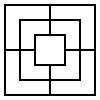
\includegraphics[width=5.5cm,height=5.5cm]{images/gameboard.png}
	\caption[Mühle Spielbrett]{Mühle Spielbrett}
\end{figure}

Zu Beginn des Spiels bekommt jeder Spieler neun, gleichfarbige Spielsteine meistens in den Farben weiß und schwarz. Das Spiel ist beendet, sobald ein Spieler nur noch zwei Spielsteine auf dem Spielbrett liegen hat oder ein Spieler keinen Spielzug mehr tätigen kann. Das Mühle Spiel lässt sich in drei Phasen gliedern:

\begin{enumerate}
\item Setzphase
\item Verschiebenphase
\item Springenphase
\end{enumerate}

\textbf{Spielregeln für die Setzphase:}

Bei der Setzphase darf jeder Spieler abwechselnd einen eigenen Spielstein auf ein Feld des Spielbrettes legen. Wenn beide Spieler ihre neun Spielsteine gesetzt haben beginnt die zweite Phase.

\textbf{Spielregeln für die Verschiebenphase:}

Jeder Spieler darf abwechselnd einen eigenen Spielstein auf ein freies, benachbartes Feld setzen. Das Feld auf das der Spielstein verschoben werden soll muss über eine Verbindungslinie mit dem aktuellen Feld auf dem der Spielstein liegt verbunden sein. Wenn ein Spieler keinen seiner verbleibenden Spielsteine bewegen kann hat der Spieler verloren.

\textbf{Spielregeln für die Springenphase:}

Sobald ein Spieler nur noch drei Spielsteine auf dem Spielbrett hat befindet sich dieser Spieler in der Springenphase. In dieser Phase darf der Spieler jede Runde einen eigenen Stein auf ein beliebiges freies Feld setzen. Wenn der Spieler nur noch zwei Spielsteine auf dem Spielbrett besitzt hat er das Spiel verloren.

\textbf{Eine Mühle bilden:}

In jeder Phase des Spiels kann ein Spieler eine Mühle bilden. Eine Mühle besteht aus drei gleichfarbigen und benachbarten Spielsteinen die auf einer Geraden liegen. Wenn ein Spieler eine Mühle bildet darf er dem gegnerischen Spieler einen Spielstein entfernen. Der entfernte Spielstein darf nicht Teil einer Mühle sein, außer alle gegnerischen Spielsteine sind Teil einer Mühle, dann darf auch ein Spielstein von einer Mühle entfernt werden.

\begin{figure}[ht]
	\centering
	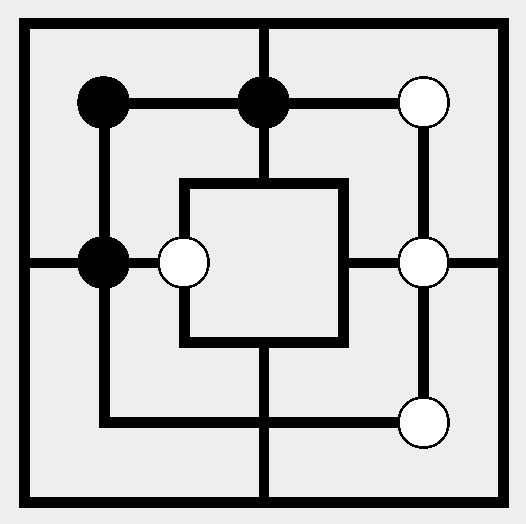
\includegraphics[width=5.5cm,height=5.5cm]{images/mill.png}
	\caption[Gebildete weiße Mühle]{Gebildete weiße Mühle}
\end{figure}

\textbf{Wissenswertes:}

Die möglichen Stellungen bei einem Mühle Spiel beträgt etwa 1,8 * 10\textsuperscript{10}. Alle möglichen Spielstellungen wurden in einer 17 GByte großen Datenbank gespeichert. Dabei verbraucht eine Stellung mit Bewertung ein Byte. Jürg Nievergelt und Ralph Gasser beweisten 1994 an der ETH Zürich das eine Partie die beidseitig korrekt gespielt wird immer unentschieden endet. Um diesen Beweis zu erbringen wurden drei Jahre lang mit Unterbrechungen auf mehreren Computern und verschiedenen Programmen Berechnungen durchgeführt.

\section{Eingesetzte Software und Programmiersprache}

\subsection{Programmiersprache Java}

Java ist eine objektorientierte Programmiersprache die 1995 von Sun Microsystems entwickelt wurde. Seit 2010 ist Sun Microsystems ein Tochterunternehmen von Oracle. Dabei ist Java eine plattformunabhängige Programmiersprache das bedeutet das die geschriebene Software sowohl auf Windows, MacOS, Linux und vielen weiteren Betriebssystemen lauffähig ist.

\subsection{GUI-Toolkit Swing}

Swing wurde ebenfalls von Sun Microsystems entwickelt und gehört seit 1998 zur Java-Runtime. Mithilfe von Swing können grafische Benutzerschnittstellen objektorientiert programmiert werden. Durch die Plattformunabhängigkeit von Swing können auch diese Anwendungen auf verschiedenen Betriebssystemen ausgeführt werden.

\subsection{Eclipse}

Eclipse ist eine quelloffene und integrierte Entwicklungsumgebung (IDE) für die Entwicklung von Software. Auch Eclipse ist plattformunabhängig einsetzbar. Für Eclipse gibt es unzählige Erweiterungen sogenannte Plugins.

\subsection{Inkscape}

Die frei verfügbare und plattformunabhängige Software Inkscape ist zur Erstellung und Bearbeitung zweidimensionaler Vektorgrafiken entwickelt worden. Vektorgrafiken haben den Vorteil das sie auf verschiedene Größen skaliert werden können ohne das diese unscharf angezeigt werden. 

\subsection{Github}  

Github ist ein Versionsverwaltungssystem mit deren Hilfe Software-Entwicklungsprojekte auf Servern bereitgestellt wird. Damit können ganze Software Teams an einem Projekt arbeiten das den gleichen Projektstand aufweist. Ein weiterer Vorteil ist die Wiederherstellung älterer Softwareversionen die als Backup dienen können.

\section{Was ist künstliche Intelligenz?}

Künstliche Intelligenz (KI) oder auch artifizielle Intelligenz (AI) genannt ist ein Teilgebiet der Informatik und versucht eine möglichst menschenähnliche Intelligenz zu simulieren. Daraus folgt das eine Software die eine künstliche Intelligenz simulieren soll Probleme eigenständig lösen kann. Durch die Kombination der beiden Fachgebiete Mathematik und Informatik kann intelligentes Verhalten auf computergestützten Systemen simuliert werden. Die Forschungs- und Entwicklungsergebnisse der KI nahm auch auf viele weitere Forschungsgebiete Einfluss vor allem in den Neurowissenschaften. Im Bereich der künstlichen Intelligenz wird zwischen einer starken KI und einer schwachen KI unterschieden:

\textbf{Starke KI:}

Durch eine starke KI soll die Intelligenz des Menschen und dessen Gedankengänge mechanisiert werden. Eine Maschine soll sich so verhalten wie ein Mensch. Weltweit wird dieses Ziel von vielen Forschungs- und Entwicklungsteams verfolgt. Gefühle wie Liebe, Trauer, Freude, Angst, ... können nur ansatzweise simuliert und nachgeahmt werden. Bisher konnte die Vision der starken KI nicht vollständig umgesetzt werden.

\textbf{Schwache KI:}

Bei der schwachen KI sollen verschiedenste Anwendungsprobleme des Menschen durch simulierte Intelligenz unterstützt und gelöst werden. Manche KI Systeme sind in der Lage durch künstliche neuronale Netze selbstständig zu lernen. Dies wird auch unter dem Begriff Deep Learning verstanden. Solche Systeme werden nicht mehr programmiert, sondern mit Hilfe von Daten trainiert. In den letzten Jahrzehnten gab es im Bereich der schwachen KI enorme Fortschritte.

\textbf{Turing-Test:}

Alan Turing ein britischer Mathematiker entwickelte im Jahr 1950 den sogenannten Turing-Test. Dabei kommuniziert ein Mensch parallel mit einem Mensch und einer Maschine zum Beispiel über ein Chat Programm. Sowohl Mensch als auch Maschine versuchen die Testperson zu überzeugen das ein realer Mensch mit ihnen kommuniziert. Wenn die Testperson am Ende der Unterhaltung nicht eindeutig bestimmen kann welcher der Gesprächspartner Mensch oder Maschine ist gilt die Maschine als intelligent. Bisher wurde der Turing-Test von keiner Maschine bestanden und KI-Experten gehen davon aus das dies in absehbarer Zeit auch nicht passieren wird.

\pagebreak

\section{Einsatzgebiete von künstlicher Intelligenz}

\subsection{Gesichtserkennung}

Einige Gebiete der künstlichen Intelligenz wird von uns Menschen heutzutage nicht mehr als künstliche Intelligenz betrachtet, da diese in unseren Alltag integriert wurden. In dieses Gebiet zählt auch die Gesichtserkennung. Für uns Menschen ist es simpel Gesichter anderer Personen zu erkennen und bekannte Gesichter Personen zuzuordnen die wir kennen. Auch wenn diese mit unterschiedlichen Lichtverhältnissen, Gesichtsausdrücken, Sonnenbrillen, etc. auftreten. Aus Sicht einer Software ist dies aber weitaus komplexer. Konkrete Anwendung findet eine Gesichtserkennungssoftware bei Sicherheitskameras die Gesichter von Verbrechern in einer Datenbank gespeichert hat und diese mit den aufgenommenen Gesichtern abgleicht. Eine weitere Anwendung befindet sich heutzutage bei vielen Menschen in der Hosentasche. Moderne Smartphones erlauben es dem Benutzer ihr Smartphone mit ihrem Gesicht zu entsperren. Allgemein wurden im Bereich der Gesichtserkennung in den letzten Jahren große Fortschritte erzielt.

\subsection{Autonomes Fahren}

Kaum ein Thema im Bereich künstlicher Intelligenz ist so populär wie das autonome Fahren. Große Unternehmen wie beispielsweise Google, Tesla, Uber und viele weitere entwickeln selbstfahrende Fahrzeuge. Heutige Fahrzeuge besitzen Software die den Sicherheitsabstand zum Vordermann automatisch einhält oder der Straßenspur folgt. Einparkhilfen sind heutzutage in vielen Fahrzeugen integriert und erleichtern dem Fahrer das einparken oder nehmen dem Fahrer gleich die ganze Arbeit ab. Aber ein komplett autonom fahrendes Fahrzeug benötigt weitaus mehr Intelligenz, da nicht jede Situation eindeutig ist und nur mit Erfahrung gemeistert werden kann. Es gibt viele Situationen wie etwa Schneefall, Baustellen, Verkehrspolizisten, etc. die hohe künstliche Intelligenz erfordert. Die Übergangszeit zwischen menschlichen auf maschinelles Fahren wird die größte Herausforderung in sich bergen. Sobald alle Fahrzeuge autonom fahren, könnten diese auch untereinander kommunizieren und den Verkehrsfluss damit positiv beeinflussen.

\begin{figure}[ht]
	\centering
	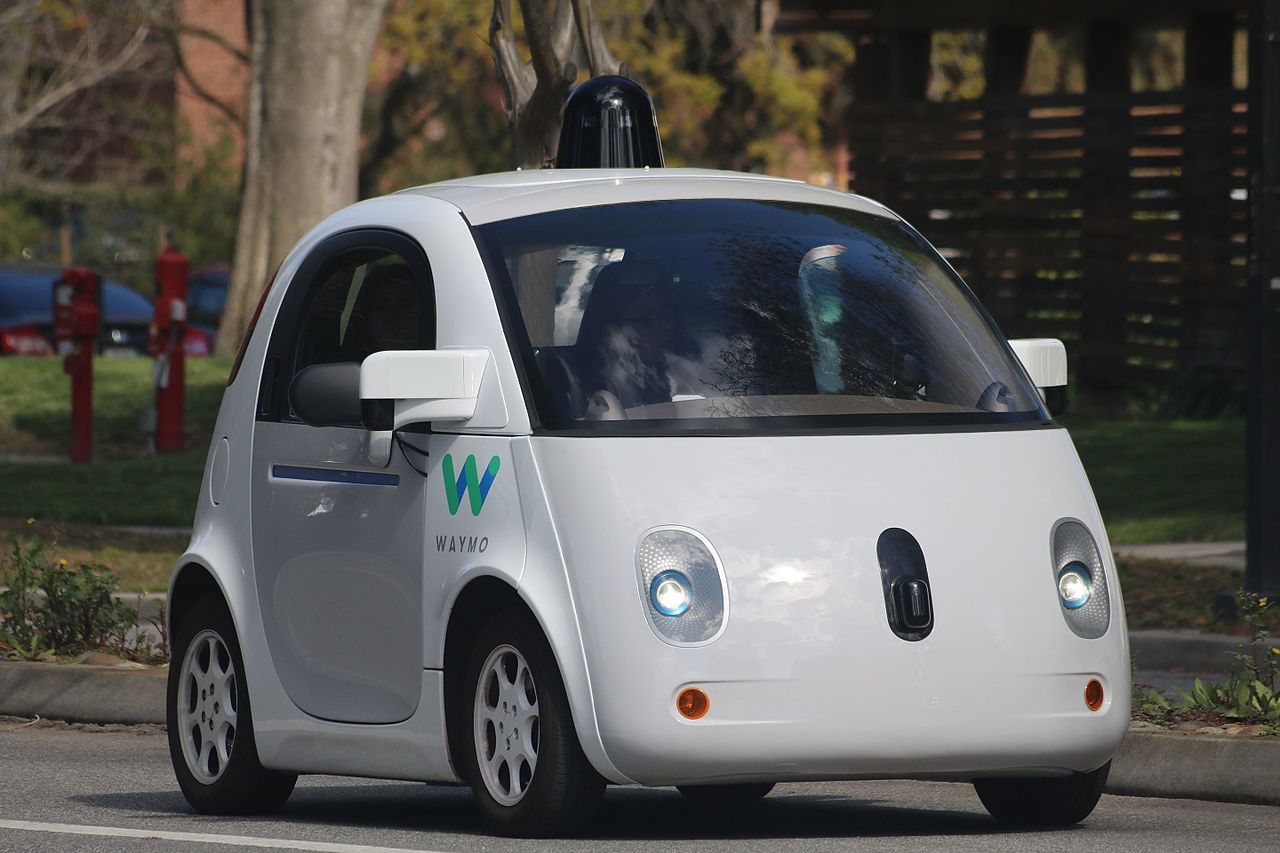
\includegraphics[width=5.5cm,height=3.5cm]{images/Waymo_self-driving_car_front_view.jpg}
	\caption[Autonomes Fahrzeug von Google]{Autonomes Fahrzeug von Google}
\end{figure}

\subsection{Robotik}

Ein weiteres großes Einsatzgebiet der künstlichen Intelligenz ist die Robotik. Schon in den 1960er Jahren kamen die ersten Roboterarme bei General Motors zum Einsatz um Aufgaben wie etwa Schweißen oder Lackieren zu übernehmen. Die Einsatzmöglichkeiten von Robotern sind vielzählig. Vor allem bei gesundheitsschädlichen oder riskanten arbeiten ersetzen Roboter immer mehr den Menschen. Im Bereich der Bombenentschärfung sind seit vielen Jahren Roboter im Einsatz.
Moderne Roboter werden immer menschenähnlicher. Hiroshi Ishiguros ist ein japanischer Ingenieursprofessor aus Osaka und konstruierte sich sein eigenes Abbild als Geminoiden.

\begin{figure}[ht]
	\centering
	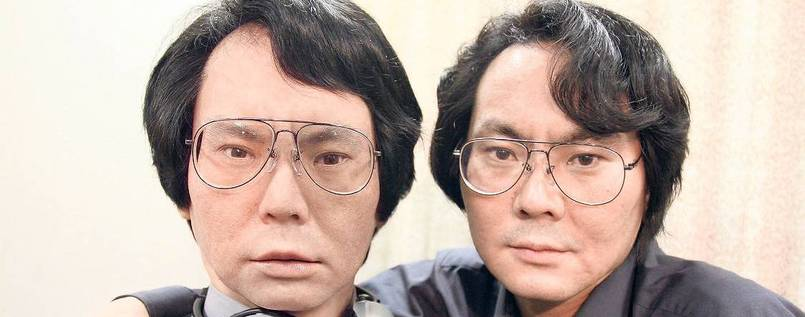
\includegraphics[width=9cm,height=4.5cm]{images/roboter.jpg}
	\caption[Hiroshi Ishiguros (rechts) und sein Roboter (links)]{Hiroshi Ishiguros (rechts) und sein Roboter (links)}
\end{figure} 

\subsection{Computerspiele}

In vielen Computerspielen ist künstliche Intelligenz heute nicht mehr wegzudenken. Kaum ein modernes 3D Computerspiel kommt ohne künstliche Intelligenz aus. Vor allem in Strategiespielen oder Shootern werden Wegfindungsalgorithmen benötigt. In populären Strategiespielen wie Dota existieren künstliche Gegner die selbst gegen Profi Spieler gewinnen. In Brettspielen wie etwa Schach, Dame, Go oder Mühle gibt es künstliche Intelligenzen die dem Menschen bereits überlegen sind und gegen die höchstens ein Unentschieden gespielt werden kann. Die programmierte Software ist dabei in der Lage viele Züge vorauszudenken. Eine künstliche Intelligenz für Mühle muss dabei viele Situationen beachten wie etwa das öffnen und schließen von eigenen oder gegnerischen Mühlen, das richtige Setzen der Spielsteine, verhindern von Zwickmühlen, etc. .  

% ---
\chapter{Aufgabenstellung}

In der objektorientierten Programmiersprache Java soll das Brettspiel Mühle programmiert werden. Die grafische Benutzerschnittstelle wird mit dem GUI-Toolkit Swing umgesetzt. Grafische Elemente wie das Spielbrett oder die Spielsteine werden mithilfe des Programms Inkscape als Vektorgrafiken erstellt. Dies hat den Vorteil das die Elemente sich der Bildschirmauflösung anpassen können ohne das diese unscharf wirken. Die GUI des Brettspiels Mühle soll sich der Bildschirmauflösung anpassen, damit Spielbrett, Spielsteine und andere grafische Elemente benutzerfreundlich dargestellt werden.

Der Kern der Software bildet die künstliche Intelligenz gegen die der Spieler antritt. Die künstliche Intelligenz muss in der Lage sein mehrere Züge nacheinander simulieren zu können. Eine selbstlernende künstliche Intelligenz ist nicht Teil des Programms. Das bedeutet die künstliche Intelligenz kann nicht trainiert werden und wird an keine Datenbank gekoppelt sein.

% ---
\chapter{Anforderungsanalyse}

\section{Aufbau von Mühle}

Eine Anforderung an die Software ist der grafische Aufbau des Mühle Spielbretts. Das Mühle Spiel soll über einen Startbildschirm gestartet werden und erreichbar sein. Die grafischen Elemente wie das Spielbrett und die Spielsteine werden als Vektorgrafiken erstellt. Diese werden dann mithilfe des GUI-Toolkit Swing in die Software integriert und angezeigt.

\begin{figure}[ht]
	\centering
	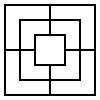
\includegraphics[width=7.5cm,height=7.5cm]{images/gameboard.png}
	\caption[Aufbau Mühle Spielbrett]{Aufbau Mühle Spielbrett}
\end{figure}

\section{Grundlegende Logik}

In allen drei Spielphasen kann eine Mühle gebildet werden dabei darf der Spieler einen gegnerischen Spielstein entfernen. Dieser Spielstein darf aber nicht Teil einer Mühle sein. Wenn alle Spielsteine des Gegners einer Mühle angehören darf auch ein Spielstein von einer Mühle entfernt werden. Spielinformationen wie die Anzahl der gespielten Runden, die verbleibenden Spielsteine, in welcher Spielphase befindet sich der Spieler und welcher Spieler ist aktuell am Zug sollen am rechten Rand des Spielbretts angezeigt werden.

\subsection{Setzphase}

In der 1.Phase der Setzphase muss jeder Spieler abwechselnd einen Spielstein auf ein freies Feld setzen dürfen. Spieler weiß darf den ersten Spielstein auf ein Feld setzen. Bei einem nicht zulässigen Spielzug soll nichts passieren bis ein gültiger Spielzug ausgeführt wird. Sobald beide Spieler ihre neun Spielsteine auf das Spielbrett gesetzt haben beginnt die 2.Phase des Mühle Spiels.

\subsection{Verschiebenphase}

In der Verschiebenphase dürfen beide Gegner abwechselnd einen Spielstein auf ein freies, benachbartes Feld setzen. Dabei müssen die Nachbarfelder des ausgewählten Feldes bekannt sein. Bei einem nicht zulässigen Spielzug soll nichts passieren bis ein gültiger Spielzug ausgeführt wird. Bei einem bereits ausgewählten Spielstein muss der Spieler in der Lage sein sich einen anderen Spielstein auswählen zu können und den Zug mit diesem weiter zu führen. Kann ein Spieler keinen Spielstein mehr verschieben hat er das Spiel verloren und der Game Over Bildschirm wird angezeigt und das Spiel wird beendet. Sobald ein Spieler nur noch drei verbleibende Spielsteine auf dem Spielbrett hat befindet sich dieser Spieler in der 3.Phase.

\subsection{Springenphase}

Wenn ein Spieler sich in der 3.Phase befindet darf er einen eigenen Spielstein auf ein beliebiges, freies Feld setzen. Bei einem nicht zulässigen Spielzug soll nichts passieren bis ein gültiger Spielzug ausgeführt wird. Bei einem bereits ausgewählten Spielstein muss der Spieler in der Lage sein sich einen anderen Spielstein auswählen zu können und den Zug mit diesem weiter zu führen. Sobald ein Spieler nur noch zwei Spielsteine besitzt hat dieser das Spiel verloren und der Game Over Bildschirm wird aufgerufen und das Spiel wird beendet.

\section{Künstliche Intelligenz}

Die künstliche Intelligenz des Mühle Spiels soll in der Lage sein mehrere Spielzüge nacheinander simulieren zu können. Es soll möglich sein verschiedene Schwierigkeitsstufen auswählen zu können. Die Schwierigkeit soll sich an der Anzahl vorraus gerechneter Spielzüge orientieren. Außerdem soll der Spieler auswählen können, ob weiß oder schwarz der KI-Gegner ist. Eine Verbindung zu einer Datenbank mit vordefinierten Spielzüge ist nicht vorgesehen. Die künstliche Intelligenz soll nicht trainiert werden können.

\section{Abgrenzung}

Die Software soll mit keiner Datenbank verbunden werden die, die bereits gespielten Spielzüge speichert und die künstliche Intelligenz trainieren kann. Es soll auch nicht möglich sein das aktuelle Mühle Spiel zu speichern oder ein bereits gespieltes Spiel zu laden. Ein rückgängig machen der Spielzüge soll nicht möglich sein. 

% ---
\chapter{Implementierung}

\section{Datenstrukturen}

\subsection{Felder}

Jedes Feld ist ein eigenes Objekt und besitzt eine eindeutige Id von 0-23. Die Felder sind wie in folgender Abbildung mit der eindeutigen Id implementiert. Zu jedem Feld gibt es eine x und y Position. Außerdem wird bei jedem Feld gespeichert von welchem Spieler ein Spielstein auf dem Feld liegt.

\begin{figure}[ht]
	\centering
	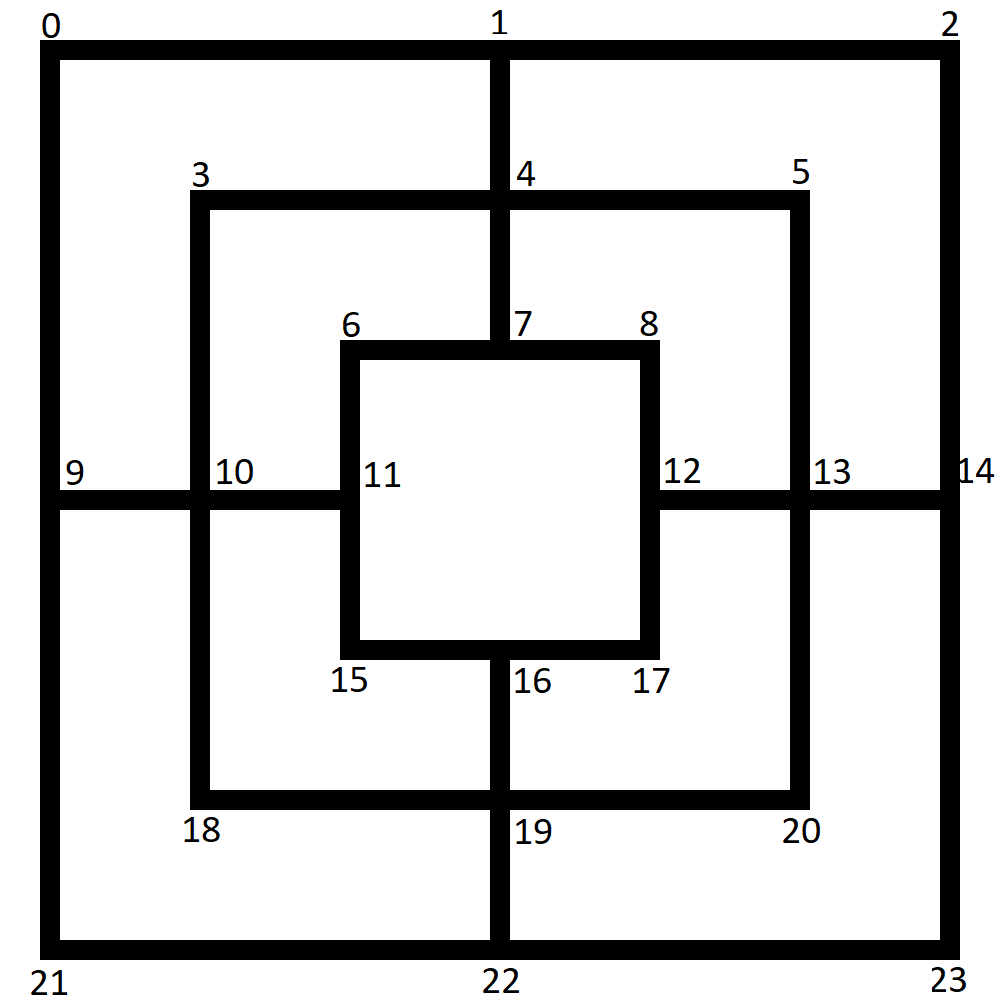
\includegraphics[width=7.5cm,height=7.5cm]{images/gameboardFields.png}
	\caption[Datenstruktur für Felder]{Datenstruktur für Felder}
\end{figure}

\subsection{Nachbarschaftsfelder}

Jedes Feld besitzt 2-4 Nachbarschaftsfelder. Dabei hat zum Beispiel das Feld mit der Id 13 die vier Nachbarschaftsfelder 5, 12, 14 und 20 (blau). Wenn ein Feld weniger als vier Nachbarschaftsfelder besitzt wie etwa das Feld mit der Id 0 werden die fehlenden Felder mit der Id -2 definiert. Daraus folgen für das Feld 0 folgende Nachbarschaftsfelder: 1, 9, -2 und -2 (grün).

\begin{figure}[ht]
	\centering
	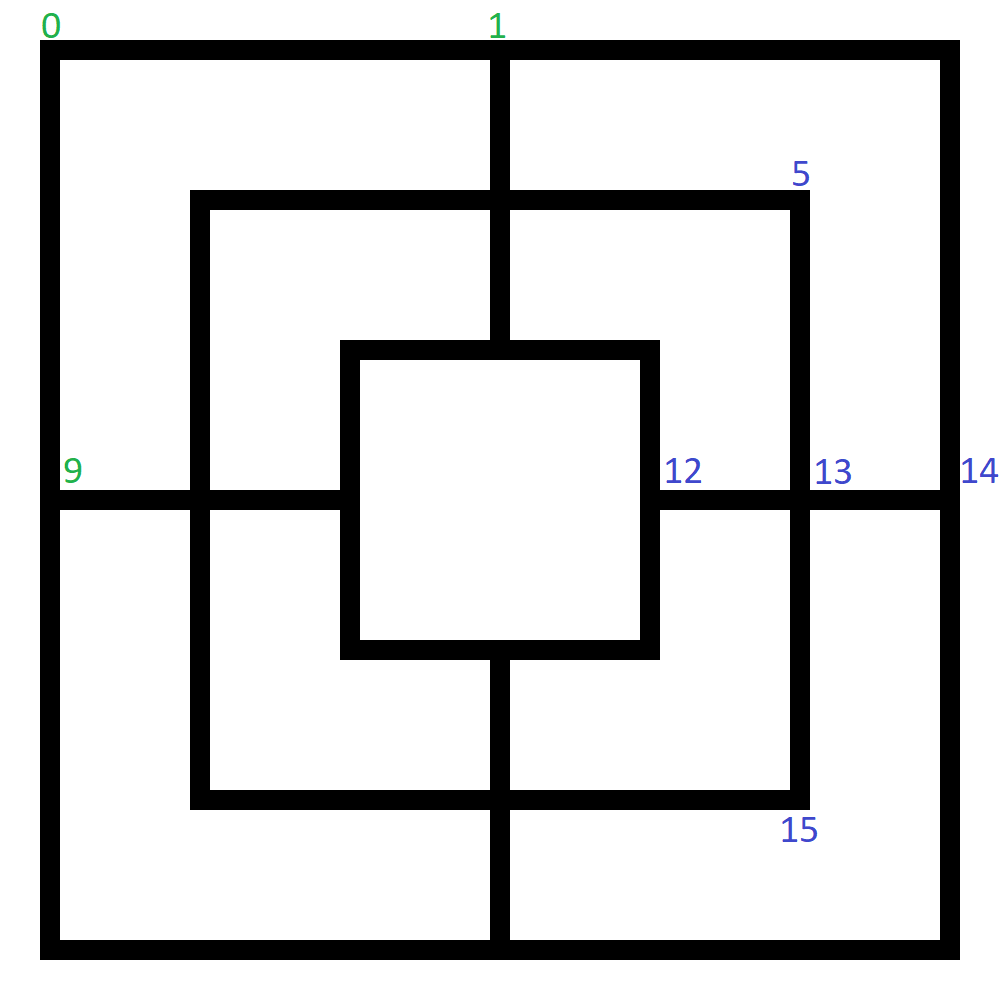
\includegraphics[width=7.5cm,height=7.5cm]{images/gameboardNeighborfields.png}
	\caption[Datenstruktur für Nachbarschaftsfelder]{Datenstruktur für Nachbarschaftsfelder}
\end{figure}

\subsection{Linien}

Insgesamt gibt es auf einem Mühle Spielbrett 16 Linien. Jede Linie hat eine eindeutige Id von 0-15. Acht Linien sind horizontal ausgerichtet und sind mit den Ids 0-7 definiert. In der Abbildung sind diese mit schwarz dargestellt. Weitere acht Linien sind vertikal ausgerichtet und sind mit den Ids 8-15 definiert. In der Abbildung sind diese mit grün hervorgehoben. Jede Linie besteht aus genau drei Feldern. Die Linie mit der Id 1 besteht aus den drei Feldern mit den Ids 3, 4 und 5. Ein Feld gehört immer zu genau zwei Linien. Das Feld 11 ist Teil der beiden Linien mit den Ids 3 (schwarz) und 10 (grün).

\begin{figure}[ht]
	\centering
	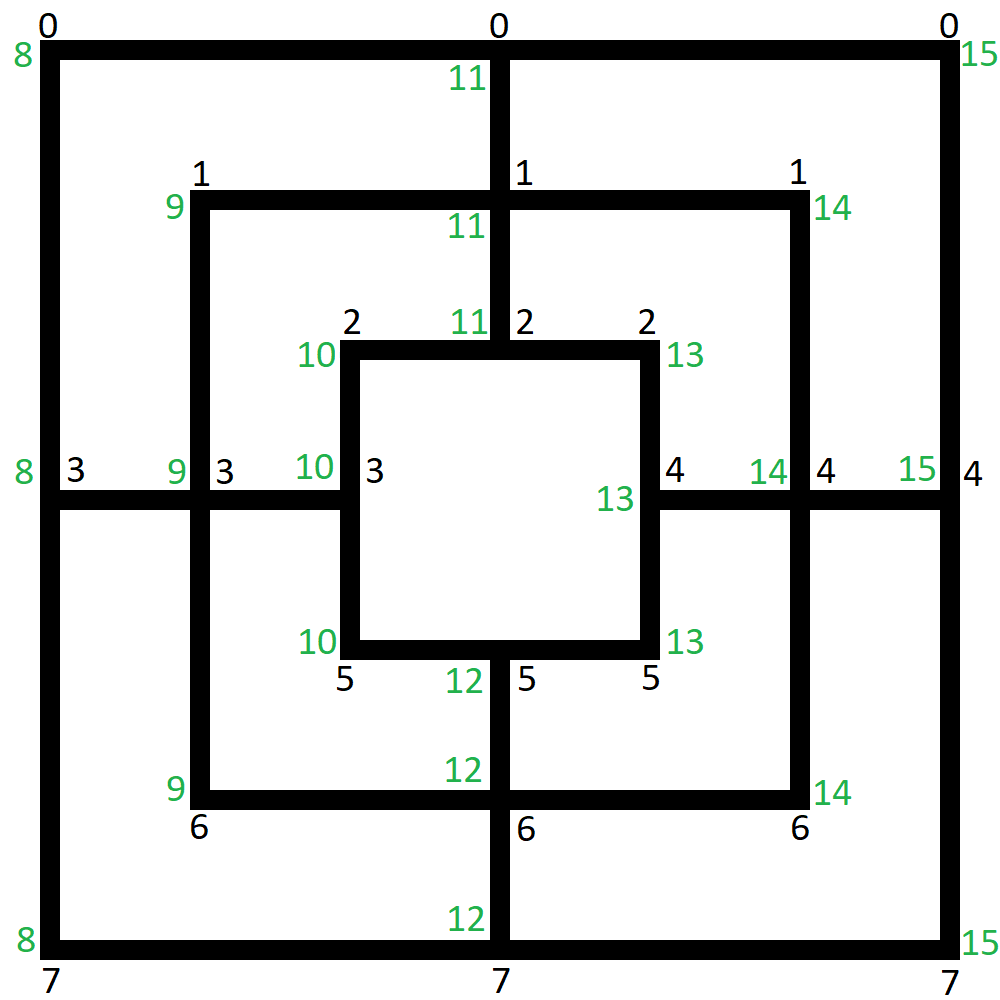
\includegraphics[width=7.5cm,height=7.5cm]{images/gameboardLines.png}
	\caption[Datenstruktur für Linien]{Datenstruktur für Linien}
\end{figure}

\subsection{Spielsteine}

Jeder Spieler hat neun gleichfarbige Spielsteine. Jeder Spielstein hat eine eindeutige Id von 0-17. Die Spielsteine mit einer geraden Id 0, 2, 4, etc. gehören zum weißen Spieler. Alle Spielsteine mit einer ungeraden Id 1, 3, 5, etc. gehören zum schwarzen Spieler. Für jeden Spielstein wird sich gemerkt, ob dieser auf dem Spielbrett liegt und ob dieser Spielstein Teil einer Mühle ist.

\subsection{Spielzüge}

Jeder Spielzug wird durch drei Variablen definiert:

\begin{enumerate}
\item from
\item to
\item remove
\end{enumerate}

In der Variable "from" wird die Feld id gespeichert von dem der Spielstein kommt. Wenn der Spielstein noch nicht im Spiel ist und noch gesetzt werden muss ist dieser Wert -1. Die Variable "to" speichert die Feld id auf die der Spielstein verschoben wird. Die Variable "remove" speichert die Feld id auf dem ein Spielstein entfernt wurde, wenn eine Mühle gelegt wurde. Wenn bei einem Spielzug kein Spielstein entfernt wird ist dieser Wert als -1 definiert. Diese Werte werden für die künstliche Intelligenz benötigt um die verschiedenen Spielzüge abbilden zu können.

\clearpage

\section{Spieler vs. Spieler}

\subsection{Setzphase}

In folgender Abbildung ist die Implementierung der 1. Phase (Setzphase) abgebildet. Zuerst wird in den Zeilen 160 - 161 überprüft welches Feld angeklickt wurde. Erst wenn ein Feld angeklickt wurde wird ein Spielzug ausgeführt. Anschließend wird in der Zeile 162 geprüft, ob der aktuelle Spieler einen Spielstein des Gegners entfernen darf oder ob der Spieler einen Spielstein setzen darf. Wenn der aktuelle Spieler einen Spielstein setzen darf wird in der Zeile 163 ermittelt, ob das angeklickte Feld frei ist. Bei einem freien Feld werden die Werte des Feldes gesetzt und in den Zeilen 176 - 178 wird geprüft ob mit dem gerade gelegten Spielstein eine Mühle gelegt wurde. Wenn ja darf der Spieler einen Spielstein des Gegners entfernen. Wenn nein ist der gegnerische Spieler am Zug. Sobald alle 18 Spielsteine gelegt wurden kommen beide Spieler in den Zeilen 183 - 186 in die 2. Phase (Verschiebenphase).

\begin{figure}[ht]
	\centering
	\includegraphics[width=17cm,height=14cm]{images/setzphaseImplementierung.png}
	\caption[1. Phase Setzphase Implementierung]{1.Phase Setzphase Implementierung}
\end{figure}

Sobald ein Spieler eine Mühle gebildet hat darf er in jeder Phase des Spiels einen gegnerischen Spielstein entfernen. Diese Funktionalität wird mit der Methode removeGamestone() erreicht. Zuerst wird in den Zeilen 389 - 390 kontrolliert, ob auf dem Feld ein gegnerischer Spielstein liegt von dem der Spieler den Spielstein entfernen möchte. Wenn dies der Fall ist wird als nächstes untersucht, ob der gegnerische Spielstein sich in einer Mühle befindet. Bei diesem Fall darf der Spielstein nicht entfernt werden, solange nicht alle gegnerischen Spielsteine in einer Mühle liegen. In den Zeilen 394 - 404 werden dann die Werte für den entfernten Spielstein und dessen Feld neu gesetzt. Anschließend ist der Gegner am Zug.

\begin{figure}[ht]
	\centering
	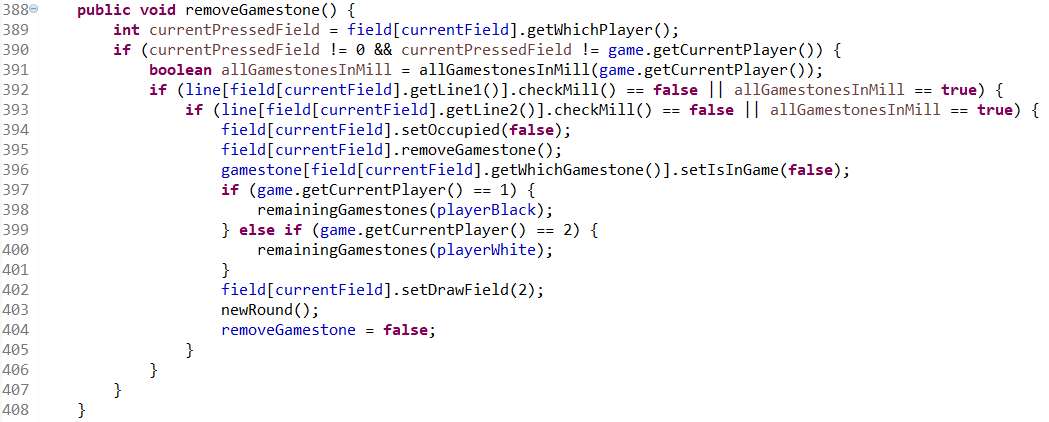
\includegraphics[width=15cm,height=8cm]{images/removeGamestoneMethode.png}
	\caption[Remove Gamestone Methode]{Remove Gamestone Methode}
\end{figure}

\subsection{Verschiebenphase}

In nachstehender Abbildung ist die Implementierung der 2. Phase (Verschiebenphase) abgebildet. In Zeile 294 - 301 wird kontrolliert, ob ein Spielstein ausgewählt wurde und es werden die Nachbarfelder des ausgewählten Feldes ermittelt. Sobald ein Spieler ein Feld ausgewählt hat kann dieser den Spielstein auf ein benachbartes Feld verschieben. Dies ist in den Zeilen 303 - 314 implementiert. Ein Spieler kann nachdem er sich für einen Spielstein entschieden hat den er verschieben möchte nochmals um entscheiden und einen anderen Spielstein auswählen. Dies wurde in den Zeilen 315 - 317 implementiert. Ab der Zeile 319 bis 330 wird entschieden ob ein Spieler in der 2. Phase bereits das Spiel verloren hat. Dies kann nur geschehen wenn der Spieler keinen Spielstein mehr bewegen kann.

\begin{figure}[ht]
	\centering
	\includegraphics[width=15cm,height=11cm]{images/verschiebenphaseImplementierungTeil1.png}
	\caption[2. Phase Verschiebenphase Implementierung Teil 1]{2.Phase Verschiebenphase Implementierung Teil 1}
\end{figure}

\begin{figure}[ht]
	\centering
	\includegraphics[width=15cm,height=7cm]{images/verschiebenphaseImplementierungTeil2.png}
	\caption[2. Phase Verschiebenphase Implementierung Teil 2]{2.Phase Verschiebenphase Implementierung Teil 2}
\end{figure}

Die Methode moveGamestone(int, int) bekommt als Übergabeparameter die ausgewählte Feld id und die Feld id auf das der Spielstein verschoben werden soll. In der Methode wird geprüft, ob das Feld auf das der Spielstein verschoben werden soll ein Nachbarfeld ist. Erst wenn dies erfüllt ist werden die Werte für die beiden Felder neu gesetzt. Im Anschluss wird noch untersucht, ob der verschobene Spielstein eine neue Mühle gebildet hat.

\begin{figure}[ht]
	\centering
	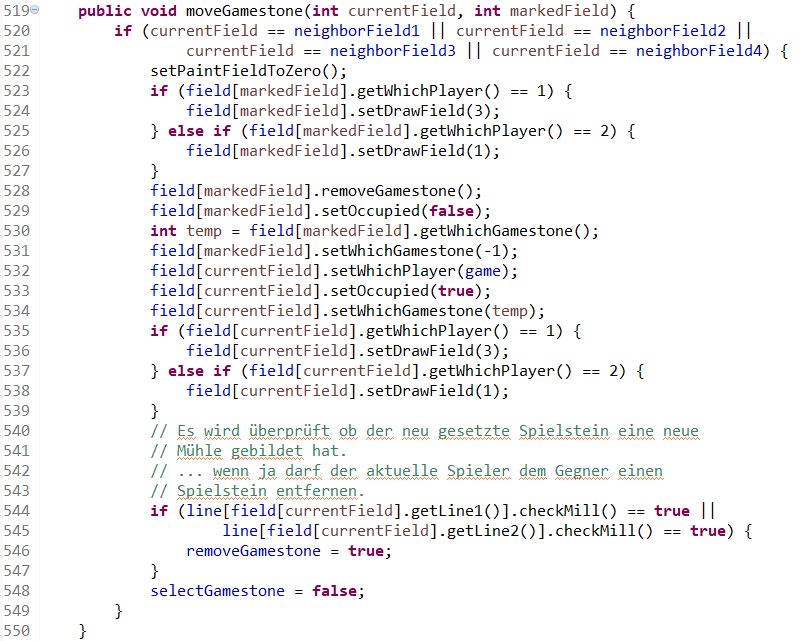
\includegraphics[width=11cm,height=10cm]{images/moveGamestoneMethode.png}
	\caption[Move Gamestone Methode]{Move Gamestone Methode}
\end{figure}

\clearpage

\subsection{Springenphase}

Die Implementierung der 3. Phase (Springenphase) ist in folgender Abbildung dargestellt. Diese Spielphase ist mit geringen Veränderungen äquivalent zu der 2. Phase. Da der Spieler sobald er in der 3. Phase ist auf ein beliebiges, freies Feld springen darf werden hier keine Nachbarfelder abgefragt. Die Methode jumpGamestone(int, int) die in Zeile 356 aufgerufen wird ist analog zu der Methode moveGamestone(int, int) mit der Ausnahme das die Nachbarfelder nicht abgefragt werden.

\begin{figure}[ht]
	\centering
	\includegraphics[width=15cm,height=13cm]{images/springenphaseImplementierung.png}
	\caption[3. Phase Springenphase Implementierung]{3.Phase Springenphase Implementierung}
\end{figure}

\clearpage

\section{Minimax-Algorithmus}

\subsection{Einführung}

Der Minimax Algorithmus ermittelt eine optimale Spielstrategie für Zwei-Personen-Nullsummenspiele mit vollständiger Information. Zu solchen Spielen zählen zum Beispiel Brettspiele wie Schach, Go, Dame oder Mühle. Der Minimax Algorithmus bildet das Kernelement der Mühle Software und der dahinter liegenden künstlichen Intelligenz. Durch die steigende Rechenleistung von Computern können diese immer mehr mögliche Züge berechnen was dazu geführt hat das die meisten Menschen ohne Mühe von Computern geschlagen werden können.

\subsection{Bewertungsfunktion}

Die Bewertungsfunktion ordnet dem Spielzug einen Wert von +1 zu, wenn Spieler A durch diesen Zug gewinnt, einen Wert von -1 wenn Spieler A verliert und 0 bei einem unentschieden. Wenn der vollständige Suchbaum bis zu seiner maximalen Tiefe aufgebaut wird spielt der Algorithmus ein perfektes Spiel. Dies ist aber nur bei einfacheren Spielen wie etwa Tic-Tac-Toe möglich. Bei komplexeren Spielen wie etwa Mühle wird der Suchbaum nur bis zu einer festgelegten Tiefe aufgebaut und anschließend ermittelt welcher Spielzug ausgeführt wird. Dabei wird die Bewertungsfunktion so modifiziert das gute Spielzüge einen hohen, positiven Wert bekommen und schlechte Spielzüge einen großen, negativen Wert. Umso größer die festgelegte Tiefe des Suchbaums ist umso schwieriger ist die künstliche Intelligenz zu schlagen. Den vollständigen Suchbaum aufzubauen würde bei komplexen Spielen zu viel Rechenleistung benötigen.

\subsection{Suchbaum Beispiel}

In folgender Abbildung ist ein Suchbaum mit der Tiefe 3 dargestellt. Der Knoten der Ebene 0 wird auch als Wurzelknoten bezeichnet und repräsentiert die aktuelle Spielsituation. Die Knoten in der tiefsten Ebene in der Abbildung also Knoten der Ebene 3 werden auch als Blattknoten bezeichnet. In Ebene 0 und 2 werden jeweils die maximalen Werte der darunterliegenden Knoten vererbt. Dabei wird die max-Methode angewendet. In Ebene 1 werden jeweils die minimalen Werte der darunterliegenden Ebene an die Knoten vererbt. Es wird die min-Methode angewendet. In folgender Abbildung wird der nächste Spielzug mit dem Wert 5 durchgeführt, da dieser den höchsten Wert aufweist.

\begin{figure}[ht]
	\centering
	\includegraphics[width=7.5cm,height=7.5cm]{images/suchbaum.png}
	\caption[Suchbaum Beispiel]{Suchbaum Beispiel}
\end{figure}

\subsection{Max Methode}

In der max Methode des Minimax Algorithmus wird in den Zeilen 108 - 110 geprüft, ob es einen Spielzug gibt mit dem die KI in den nächsten Spielrunden sicher gewinnen kann. Wenn dies der Fall ist wird der Wert -1000 als Gewicht angenommen und an den Wurzelknoten zurückgegeben. In den Zeilen 111 - 114 werden die Spielzüge in der tiefsten Ebene bewertet und das Gewicht zurückgegeben. Die Zeilen 116 - 119 sind zur Ermittlung der verfügbaren Felder implementiert die in einer Liste eingetragen werden. Wenn diese Liste leer ist, ist kein weiterer Spielzug möglich und es wird wieder das Gewicht -1000 zurückgegeben. Ab der Zeile 120 werden dann die möglichen Spielzüge mithilfe der Funktion placeAMove(move, player) berechnet. In den Zeilen 123 - 129 wird dann das maximale Gewichte ermittelt und an die oberen Ebenen des Spielbaumes weiter gegeben bis dieser im Wurzelknoten angekommen ist. In der Funktion replaceAMove(move, player) werden dann die gesetzten Werte wieder zurückgesetzt und das Spielbrett zurückgebaut um den nächsten Spielzug berechnen zu können. 

\begin{figure}[ht]
	\centering
	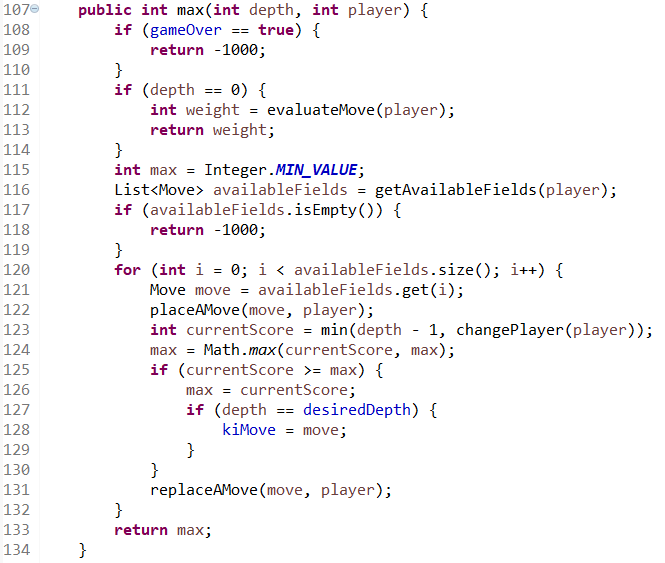
\includegraphics[width=10cm,height=7.5cm]{images/maxMethode.png}
	\caption[Max Methode Implementierung]{Max Methode Implementierung}
\end{figure}

\subsection{Min Methode}

Die min Methode des Minimax Algorithmus ist fast äquivalent zu der max Methode implementiert. Hier werden positive Gewichte weitergegeben, da die min Methode die gegnerischen Spielzuggewichte ausführt. Die max Methode führt die eigenen Spielzüge durch. Hier werden ab der Zeile 83 die möglichen Spielzüge berechnet und das minimale Gewichte ermittelt und an die oberen Ebenen des Spielbaumes weiter gegeben.

\begin{figure}[ht]
	\centering
	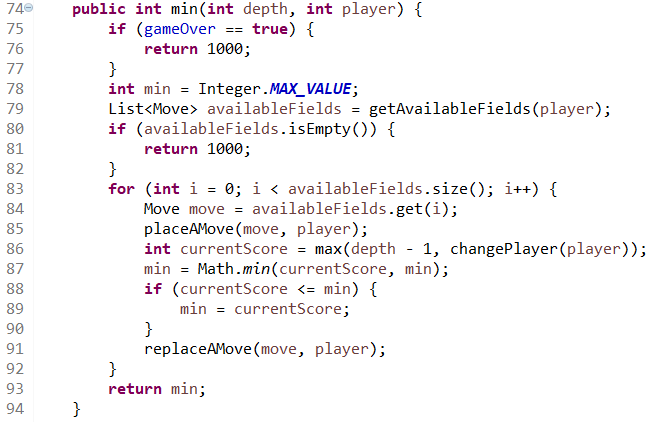
\includegraphics[width=12.5cm,height=10cm]{images/minMethode.png}
	\caption[Min Methode Implementierung]{Min Methode Implementierung}
\end{figure}

\clearpage

\subsection{Mühle Bewertungsfunktion}

Jeder Spielzugknoten der in der untersten Ebene des Spielbaumes liegt wird durch verschiedene Spielfaktoren ausgewertet. Da der Spielbaum bei Mühle nicht komplett aufgebaut und nur bis zu einer bestimmten Tiefe erstellt werden kann reicht es nicht aus die Spielzüge durch +1 (Gewonnen), 0 (Unentschieden) und -1 (Verloren) auszuwerten. Dies kann nur bei einfacheren Brettspielen wie zum Beispiel Tic-Tac-Toe realisiert werden. Der Spielausgang ist in den meisten Berechnungen im Spielbaum des Brettspiels Mühle nicht vorher abzusehen. Deshalb erfordert es eine umfangreichere Bewertungsfunktion die verschiedene Faktoren des Mühle Spiels berücksichtigt. Die folgende Tabelle stellt die Gewichtung der implementierten Faktoren dar.

\begin{table}[H]
	\renewcommand{\arraystretch}{2}
	\begin{tabular}{|c||c||c|}
	\hline
	Nummer & Faktor & Gewichtung \\ \hline \hline
	1 & eigene Mühle & +15 \\ \hline
	2 & geg. Mühle & -10 \\ \hline
	3 & mögliche Züge & mögliche Züge * 2 \\ \hline
	4 & geg. mögliche Züge & geg. mögliche Züge * (-2) \\ \hline
	5 & eigene verbleibende Spielsteine & verbleibende Spielsteine * 7 \\ \hline
	6 & geg. verbleibende Spielsteine & geg. verbleibende Spielsteine * (-7) \\ \hline
	\end{tabular}
	\caption[Faktorgewichtungen]{Faktorgewichtungen}
\end{table}

\subsection{Rechenaufwand}

Je tiefer der Spielbaum erstellt wird umso mehr Spielbretter werden mithilfe des Minimax Algorithmus aufgebaut. Ab der Tiefe 5 wird deutlich das der Rechenaufwand zum Aufbau des Spielbaums deutlich steigt und die Anwendung reagiert nicht mehr in Echtzeit und benötigt eine gewisse Zeit zur Berechnung. Die folgende Tabelle zeigt die Anzahl der erstellten Spielbretter beim ersten Spielzug der KI. Die Anzahl der erstellten Spielbretter wird unter anderem durch die unterschiedlichen Faktoren des Mühle Spiels beeinflusst. 

\begin{table}[H]
	\centering
	\renewcommand{\arraystretch}{2}
	\begin{tabular}{|c||c||c|}
	\hline
	Tiefe & Anzahl erstellter Spielbretter & Spielmodus \\ \hline \hline
	1 & 24 & \\ \hline 
	2 & 576 & Leicht \\ \hline
	3 & 12720 & \\ \hline 
	4 & 267744 & Normal \\ \hline
	5 & 5.368.224 & \\ \hline 
	6 & 102.277.344 & Schwer \\ \hline
	7 & 1.846.641.504 & \\ \hline
	\end{tabular}
	\caption[Rechenaufwand]{Rechenaufwand}
\end{table}

\chapter{Bedienungsanleitung}

\section{Programm Ausführung}

Die Mühle Software wurde mit der Programmiersprache Java entwickelt. Zum ausführen der Software wird deshalb eine Java Runtime Enviroment benötigt. Diese kann zum Beispiel unter "http://java.sun.com" heruntergeladen und installiert werden. Nähere Informationen zur Installation von Java befinden sich ebenfalls auf dieser Seite.

Die eigentliche Software ist in ausführbarer .jar Form auf der CD. Durch Klick auf diese Datei wird der Startbildschirm des Mühle Programms gestartet. Die Quelldateien und Bilddateien befinden sich ebenfalls auf der CD in einem separaten Ordner. Die Quelldateien können in Eclipse importiert und dort eingesehen werden. Dafür muss der komplette Projektordner in Eclipse importiert werden.

\clearpage

\section{Startbildschirm}

Im Startbildschirm kann ausgesucht werden ob der weiße oder schwarze Spieler die KI spielt. Wenn keine der beiden ausgewählt wurde können zwei reale Spieler gegeneinander spielen. Der weiße Spieler fängt immer an. Es gibt drei unterschiedliche Schwierigkeitsgrade:

\begin{enumerate}
\item Leicht
\item Normal
\item Schwer
\end{enumerate}

Beim Schwierigkeitsgrad Leicht rechnet der KI Gegner 2 Spielzüge vorraus. Bei Normal kann der KI Gegner 4 Spielzüge vorraus rechnen und bei Schwer 6 Spielzüge. Wenn der Schwierigkeitsgrad Schwer ausgewählt wird braucht die KI mehr Zeit um den nächsten Spielzug zu berechnen und die Anwendung läuft nicht mehr in Echtzeit. Deshalb kann es dort zu Verzögerungen kommen und der Spieler muss warten bis er seinen nächsten Spielzug tätigen kann. Wenn auf den Button Spiel beenden geklickt wird, wird die komplette Software beendet. Mit einem Klick auf den Button Spiel starten kann ein neues Spiel mit den ausgewählten Einstellungen gestartet werden.

\begin{figure}[ht]
	\centering
	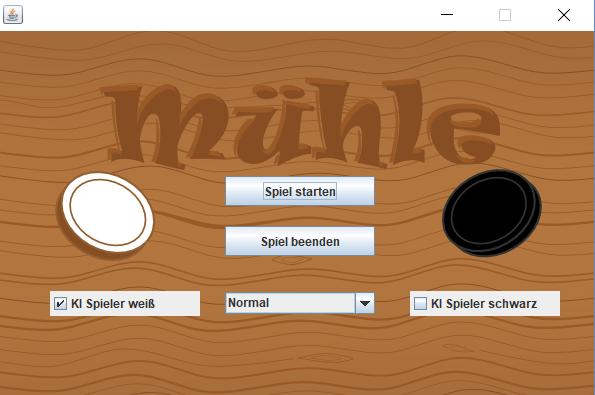
\includegraphics[width=12.5cm,height=7.5cm]{images/MuehleStartbildschirm.png}
	\caption[Mühle Startbildschirm]{Mühle Startbildschirm}
\end{figure}

\section{Mühle Spielbewegungen}

Um einen Spielstein zu setzen muss auf das entsprechende Feld geklickt werden auf dem der Spielstein gesetzt werden soll. Ein schwarzer Rahmen zeigt den letzten Spielzug des schwarzen Spielers an. Ein grüner Rahmen zeigt den letzten Spielzug des weißen Spielers an. Eine rote Umrandung zeigt an das auf diesem Feld ein Spielstein entfernt wurde. In der Verschiebenphase muss zuerst der Spielstein angeklickt werden mit dem gefahren wird und danach das Zielfeld auf das der Spielstein gesetzt werden soll. In der Springenphase ist dies äquivalent und es kann auf jedes freie Feld gesprungen werden.

\begin{figure}[ht]
	\centering
	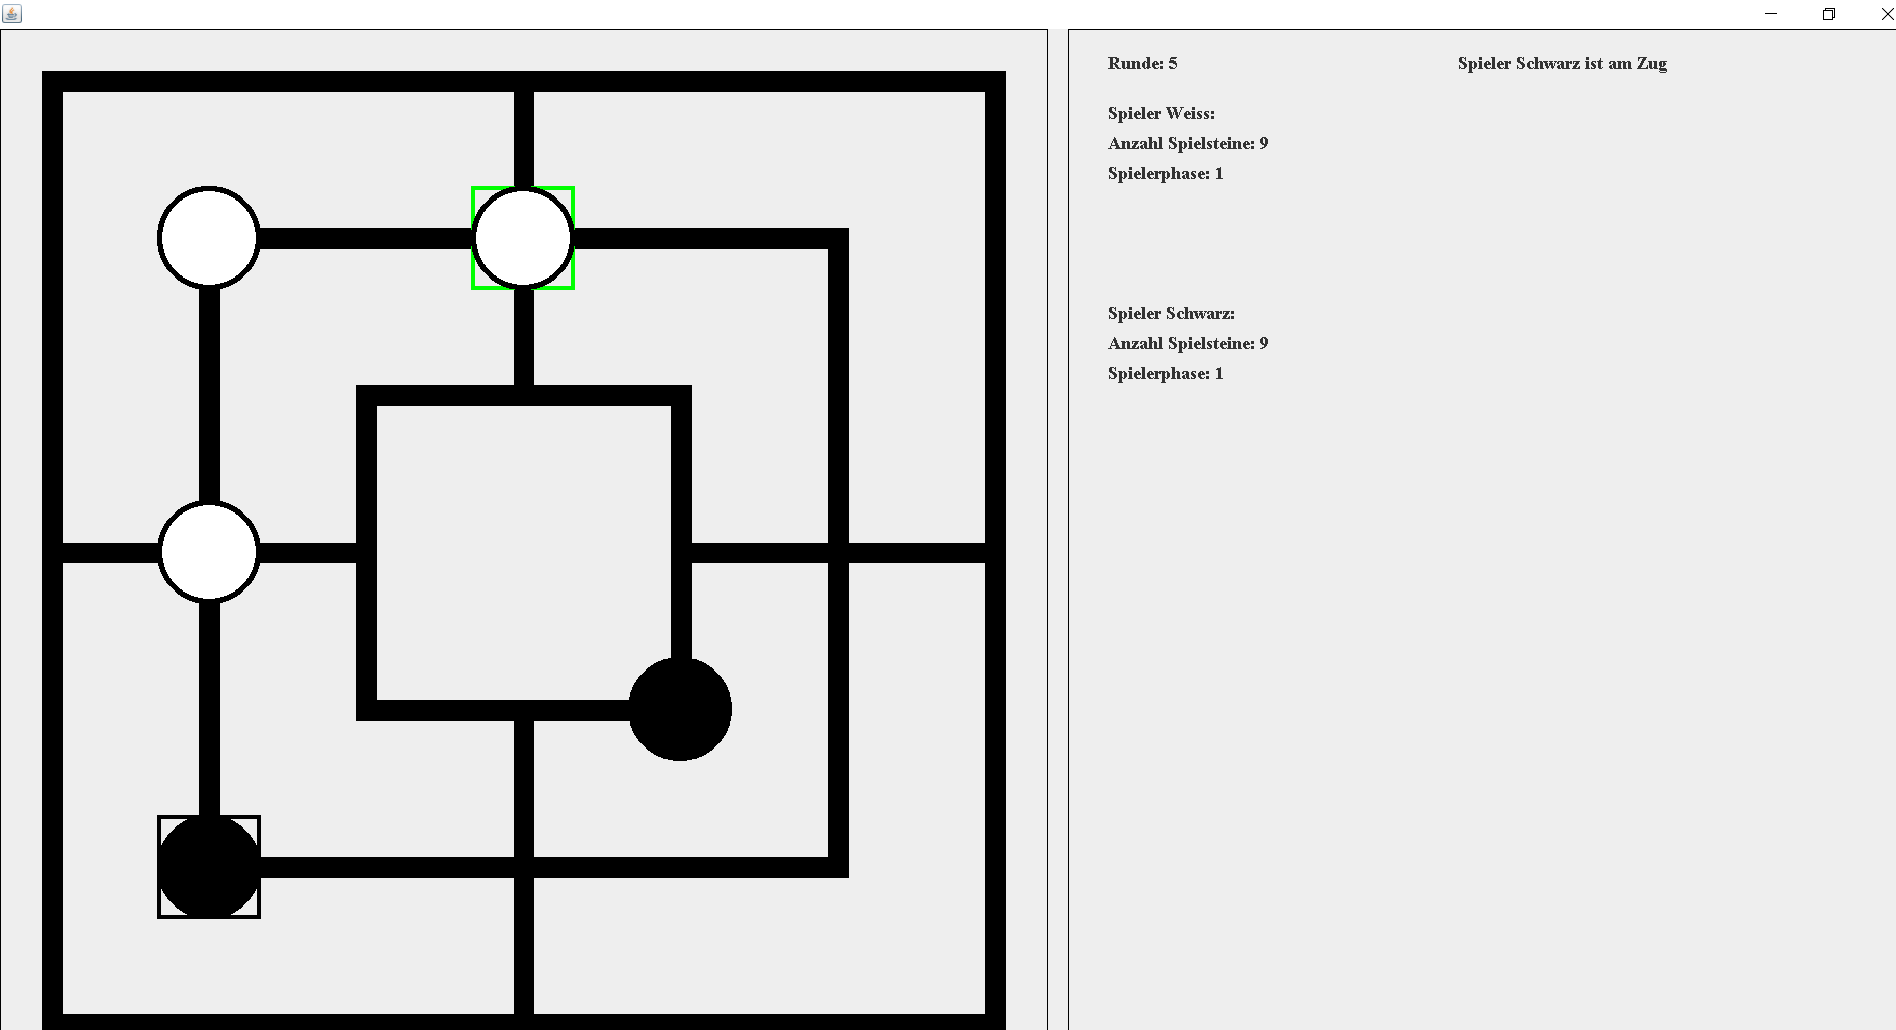
\includegraphics[width=16.0cm,height=8.5cm]{images/MuehleSpiel.png}
	\caption[Mühle Spielbildschirm]{Mühle Spielbildschirm}
\end{figure}

Sobald ein Spieler gewonnen hat, weil der Gegner nur noch zwei Spielsteine hat oder mit keinem Spielstein mehr fahren kann wird ein Fenster mit einem Siegertext geöffnet. Mit einem Klick auf den Hauptmenü Button wird wieder der Startbildschirm geöffnet.

\begin{figure}[ht]
	\centering
	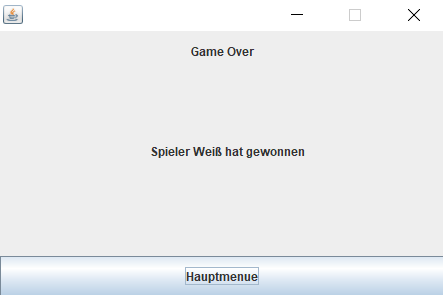
\includegraphics[width=7cm,height=5cm]{images/Endbildschirm.png}
	\caption[Mühle Endbildschirm]{Mühle Endbildschirm}
\end{figure}

% ---
\chapter{Fazit und Ausblick}

Das Fazit meiner Projektarbeit ist das die Berechnung des Minimax Algorithmus für Zwei-Personen Brettspiele wie etwa Mühle positiv ausfällt. Die Rekursion des Algorithmus ist auch in tieferen Ebenen effizient und gibt mit der passenden Bewertungsfunktion gute und sinnvolle Spielzüge zurück. Mit steigender Tiefe des Spielbaums werden die Spielzüge des KI-Gegners immer ausgereifter und stellen selbst geübte Mühle Spieler vor einige Schwierigkeiten.

Künstliche Intelligenz wird in Zukunft in unserem alltäglichen Leben immer mehr unbewusst Platz einnehmen. Schon heute nehmen wir manche künstliche Intelligenz nicht mehr als solche wahr. Viele Forschungs- und Entwicklerteams versuchen künstliche Intelligenzen in Alltagsgegenstände zu integrieren wie etwa Autos um den Traum vom autonomen Fahren zu ermöglichen. Diese Entwicklungen sind wichtig und haben auch ihren Stellenwert. Dennoch darf nicht vergessen werden das die Technologie von Menschen kontrollierbar bleiben muss. Erst dieses Jahr musste ein Forschungsteam von Facebook zwei Bots eines KI-Systems abschalten, da diese ihre eigene Geheimsprache entwickelten. An solchen Entwicklungen wird das Potenzial künstlicher Intelligenz sichtbar und das die Forschungen in diesem Bereich noch lange nicht zuende sind.

\end{document}